
\section{Artificial Immune Network}

\begin{frame}
\huge \textbf{{Artificial Immune Network(AIN)}}
\large {Zhong,Wenfeng}
\end{frame}

\begin{frame}{What is AIN?}
\begin{itemize}
\item {\textbf{The artificial immune network model(AIN)} regards artificial immune system(AIS) as a network structure composed of nodes (lymphocytes). Through the information transfer and interaction between nodes, the immune system functions such as recognition, response, and memory are achieved.}
\item {\textbf{applied to} data mining , time series prediction, pattern recognition, optimization, fault detection ...}
\end{itemize}
\end{frame}

\begin{frame}{Features}
\begin{itemize}
\item Realize and express the results of data information processing in the form of a network;
\item Deal with large amounts of data in decentralized organizations;
\item Achieve sustainable learning in the form of a dynamic network;
\item Threshold-based information processing;
\item Quickly process data information in a parallel, distributed manner.
\end{itemize}
\end{frame}

\begin{frame}{Relationship of AIN Models}
\begin{center}
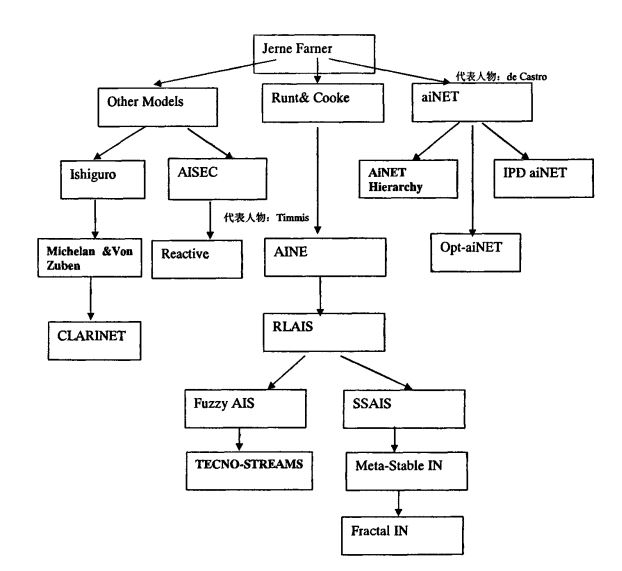
\includegraphics[scale=0.64]{img/relationship_of_AIN.JPG}
\end{center}
\end{frame}


\begin{frame}{Basic framework of AIN}
\begin{center}
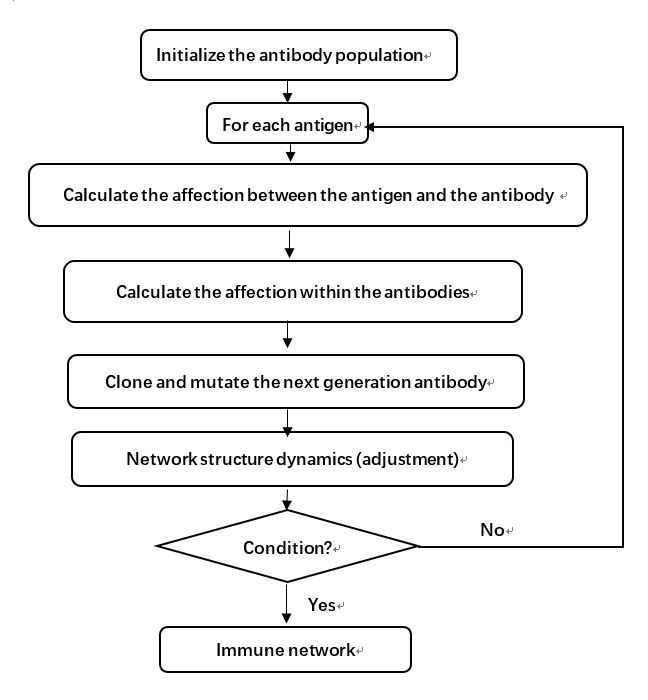
\includegraphics[scale=0.55]{img/basic_framework_of_AIN.JPG}    
\end{center}
\end{frame}

\begin{frame}{Applications of AIN}{multimodal function optimization}
\begin{columns}[c] 
\column{.5\textwidth} 
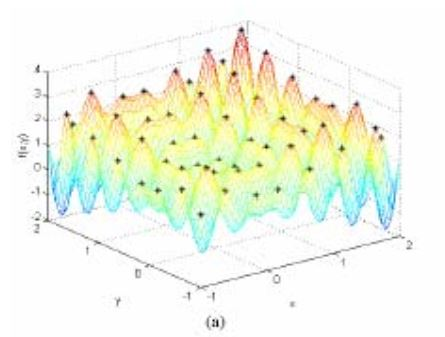
\includegraphics[scale=0.6]{img/multimodal_function_optimization_AIN.JPG}
\column{.5\textwidth} 
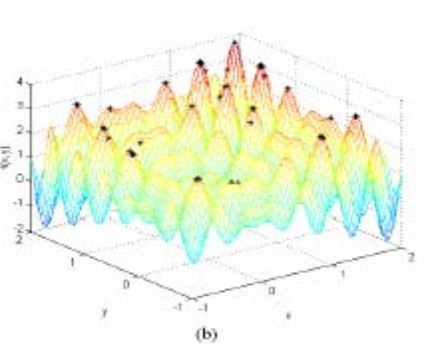
\includegraphics[scale=0.6]{img/multimodal_function_optimization_clonalg.JPG}
\end{columns}
\end{frame}

\begin{frame}{Applications of AIN}{associative classification}
\begin{columns}[c] 
\column{.5\textwidth} 
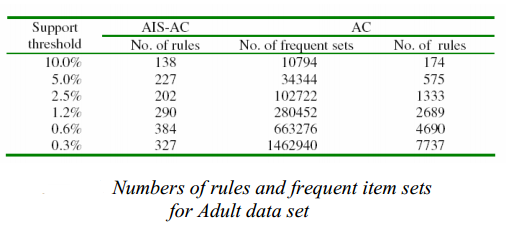
\includegraphics[scale=0.45]{img/associative_classification_table.png}
\column{.5\textwidth} 
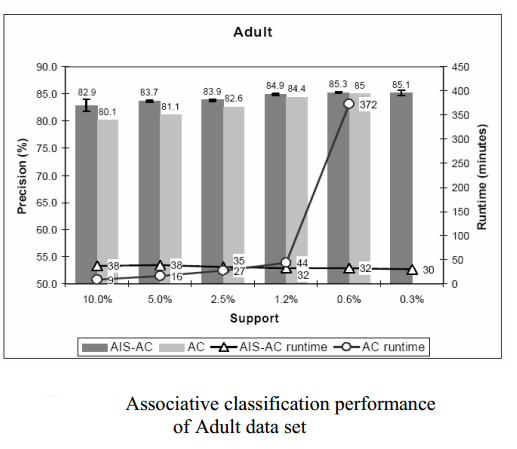
\includegraphics[scale=0.3]{img/associative_classification_figure.png}
\end{columns}
\end{frame}


\begin{frame}
\centering \Huge \textbf{Thank You!}
\end{frame}
